\chapter{Covid-19 Task Force}
\label{chap:covid}

At the start of the Covid-19 pandemic (March-April 2020), I took part in an Inria task force that was created to provide scientific expertise to external stakeholders.
In particular, we worked with the Assistance Publique-Hôpitaux de Paris (AP-HP), in order to help the AP-HP better understand and model the progression of the Covid-19 epidemic in the four central departments of the Paris.
We proposed a model that used emergency call regulation data, such as the total number of calls, number of calls resulting in the dispatch of an emergency vehicle, number of patients hospitalized with Covid-19, and number of patients in Intensive Care Units (ICUs), as input data to estimate the progression of the epidemic.
Using this model, we were able to show that there were strong discrepancies between the different departments, and that it was possible to predict the evolution of the number of cases from the emergency call regulation data.

The rest of this appendix comprises the journal article~\citep{gaubert2020}, published in the \emph{Comptes-Rendus Mathématique} of the French Academy of Sciences, that describes this work in detail.

\includepdf[pages={2-}]{covid/covid.pdf}
